% ### Erste Seite der Nietverbindungen ###
\centering
\section*{\myul{Nietverbindungen}}

\begin{tikzpicture}[remember picture, overlay]

% --- ERSTE REIHE: Am Seitenursprung anfangen
\setlength{\rowheight}{50mm}

    % X1) Eigene Zeile für die Überschrift
    \Tile{X1}{([xshift=10mm, yshift=-16mm]current page.north west)}{190mm}{18mm}
        {
            Zusätzliche Sicherheitsvielfache bei Nietverbindungen aufgrund von Spannungskonzentrationen an Nietlöchern:\\
            $j_{s1} = \text{1,15}$\,; Sitze, Liegebetten, Gurte: $j_{s2} = \text{1,33}$\,; Gussbauteile: $j_{s3} = \text{1,25}$\\[2.0ex]
            \titlebf{Schubbelastung}
        }{0}{0}{0}{0}

    % A1) Erste Kachel unten anbauen
    \setlength{\cellwidth}{42mm}
    \Tile{A1}{(X1.south west)}{\cellwidth}{\rowheight}
        {
            \vspace{-\TileSep}
            \titlerm{Blechdicke}\\ \vspace{-3mm}
            \begin{equation*}
                \frac{d}{s}\stackrel{!}{<} \text{5,5}\quad\Leftrightarrow\quad s \stackrel{!}{>} \frac{d}{\text{5,5}}
            \end{equation*}%
            \vspace{-3mm}
            {\scriptsize
            \begin{align*}
                d &= \text{Nietdurchmesser} \\
                s &= \text{Minimale Blechdicke}
            \end{align*}
            }%
            \vspace{-1mm}
            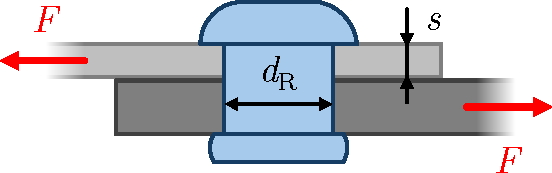
\includegraphics[width=\dimexpr\cellwidth-2\TileSep]{images/niete.pdf}
        }{0}{1}{1}{0}

    % B1) Zweite Kachel rechts anbauen
    \setlength{\cellwidth}{48mm}
    \Tile{B1}{(A1.north east)}{\cellwidth}{\rowheight}
        {
            \vspace{-\TileSep}
            \titlerm{Abscheren des Niets}\\ \vspace{-3.5mm}
            \begin{equation*}
                P_\text{B} \stackrel{!}{\leq} P_\text{V} = R_\text{C}~\frac{\pi~d_\text{R}^2}{4}~n~m
            \end{equation*}%
            \vspace{-3mm}
            {\scriptsize
            \begin{align*}
                P_\text{B} &= \text{Bemessungs-Bruchlast}                  \\
                P_\text{V} &= \text{Versagenslast}                         \\
                R_\text{C} &= \text{Scherfestigkeit}                       \\
                d_\text{R} &= \text{Nietschaftdurchmesser}                 \\
                           &= d \text{ (Pass- und Blindniet)}              \\
                           &= d + \text{0,05\,mm} \text{ (Geschlag. Niet)} \\
                n          &= \text{Nietzahl}                              \\
                m          &= \text{Schnittigkeit}
            \end{align*}
            }
        }{0}{1}{1}{0}

    % C1) Dritte Kachel rechts anbauen
    \setlength{\cellwidth}{42mm}
    \Tile{C1}{(B1.north east)}{\cellwidth}{\rowheight}
        {
            \vspace{-\TileSep}
            \titlerm{Scherbruch (Blech)}\\ \vspace{-3.5mm}
            \begin{equation*}
                P_\text{B} \stackrel{!}{\leq} P_\text{V} = 2~e~s~R_\text{C}
            \end{equation*}%
            \vspace{-3mm}
            {\scriptsize
            \begin{align*}
                P_\text{B} &= \text{Bemessungs-Bruchlast}    \\
                P_\text{V} &= \text{Versagenslast}           \\
                e          &= \text{Randabstand}             \\
                s          &= \text{Dünnste Blechdicke}      \\
                R_\text{C} &= \text{Scherfestigkeit (Blech)}
            \end{align*}
            }
        }{0}{1}{1}{0}

    % D1) Vierte Kachel rechts anbauen
    \setlength{\cellwidth}{58mm}
    \Tile{D1}{(C1.north east)}{\cellwidth}{\rowheight}
        {
            \vspace{-\TileSep}
            \titlerm{Ausreißen durch Spalten}\\ \vspace{-4mm}
            \begin{equation*}
                \resizebox{\cellwidth-2\TileSep}{!}{%
                $\displaystyle P_\text{B} \stackrel{!}{\leq} P_\text{V} = \left(e-\frac{d}{2}\right)\,s~\text{min}\!
                \begin{cases}
                    R_\text{m} \\
                    \text{1,5}~R_\text{p0,2}
                \end{cases}$}
            \end{equation*}%
            \vspace{-4mm}
            {\scriptsize
            \begin{align*}
                P_\text{B}    &= \text{Bemessungs-Bruchlast}    \\
                P_\text{V}    &= \text{Versagenslast}           \\
                e             &= \text{Randabstand}             \\
                d             &= \text{Bohrungsdurchmesser}     \\
                s             &= \text{Dünnste Blechdicke}      \\
                R_\text{m}    &= \text{Bruchfestigkeit (Zug)}   \\
                R_\text{p0,2} &= \text{Dehngrenze}
            \end{align*}
            }
        }{0}{0}{1}{0}

\end{tikzpicture}